\documentclass{beamer}
\usepackage{graphicx, import, tikz, pgf}

%\usepackage{amsmath}


\newenvironment{frcseries}{\fontfamily{frc}\selectfont}{}
\newcommand{\textfrc}[1]{{\frcseries#1}}

%\newcommand{\mathfrc}[1]{\text{\textfrc{#1}}}

\graphicspath{{../common/images/}}

\beamertemplatetransparentcovered
\usetheme{JuanLesPins}
\useinnertheme{circles}
\useoutertheme[subsection-false]{smoothbars}

\title{The multi-species coalescent}
\author{Alexei Drummond, a.drummond@auckland.ac.nz \\ \quad \\ Centre for Computational Evolution}
\date{}

\begin{document}

%Slide1
\frame{\titlepage}

%Section1 Outline
\section[Outline]{}

% TABLE OF CONTENTS
\frame{\tableofcontents}

\section{Trees}

\subimport{../common/slides/}{Slide_DarwinsTree}


% TYPES OF PHYLOGENIES AND REPRESENTATIONS
%\begin{frame}
%\frametitle{Types of phylogenies and representations}
%
%\begin{columns}
%
%\column{0.66\textwidth}
%
%\begin{centering}
%
%rooted trees
%
%\end{centering}
%
%\column{0.34\textwidth}
%
%\begin{centering}
%
%unrooted tree
%
%\end{centering}
%
%\end{columns}
%
%\begin{columns}[b]
%
%\column{0.33\textwidth}
%
%\begin{centering}
%
%% Auto-generated from TikzTree.java
%% xScale=-0.5 yScale=-0.5 offset=0.2
%% scalebar=null
%% options=[ultra thick]
%% newick=((((A: 1, B: 1): 1, C: 2): 1, D: 3): 1, E: 4);
%\begin{tikzpicture}[ultra thick]
%
%\node at (0.2, 0.0) {A};
%\node at (0.2, -0.5) {B};
%\draw (0.0, 0.0) -- (-0.5, 0.0) -- (-0.5, -0.25);
%\draw (0.0, -0.5) -- (-0.5, -0.5) -- (-0.5, -0.25);
%\node at (0.2, -1.0) {C};
%\draw (-0.5, -0.25) -- (-1.0, -0.25) -- (-1.0, -0.625);
%\draw (0.0, -1.0) -- (-1.0, -1.0) -- (-1.0, -0.625);
%\node at (0.2, -1.5) {D};
%\draw (-1.0, -0.625) -- (-1.5, -0.625) -- (-1.5, -1.0625);
%\draw (0.0, -1.5) -- (-1.5, -1.5) -- (-1.5, -1.0625);
%\node at (0.2, -2.0) {E};
%\draw (-1.5, -1.0625) -- (-2.0, -1.0625) -- (-2.0, -1.53125);
%\draw (0.0, -2.0) -- (-2.0, -2.0) -- (-2.0, -1.53125);
%
%\end{tikzpicture}
%
%\end{centering}
%
%\bigskip{}
%
%\begin{centering}
%
%(a) cladogram
%
%\end{centering}
%
%\column{0.33\textwidth}
%
%\begin{centering}
%
%% Auto-generated from TikzTree.java
%% xScale=-4.0 yScale=-0.5 offset=0.2
%% scalebar=scalebar{size= 0.1 visible=true}
%% options=[ultra thick]
%% newick=((((A: 0.1, B: 0.2): 0.12, C: 0.3): 0.123, D: 0.4): 0.1234, E: 0.5);
%\begin{tikzpicture}[ultra thick]
%
%\node at (-0.2, 0.0) {A};
%\node at (0.2, -0.5) {B};
%\draw (-0.4, 0.0) -- (-0.8, 0.0) -- (-0.8, -0.25);
%\draw (0.0, -0.5) -- (-0.8, -0.5) -- (-0.8, -0.25);
%\node at (0.12000000000000001, -1.0) {C};
%\draw (-0.8, -0.25) -- (-1.28, -0.25) -- (-1.28, -0.625);
%\draw (-0.08, -1.0) -- (-1.28, -1.0) -- (-1.28, -0.625);
%\node at (0.028000000000000025, -1.5) {D};
%\draw (-1.28, -0.625) -- (-1.772, -0.625) -- (-1.772, -1.0625);
%\draw (-0.172, -1.5) -- (-1.772, -1.5) -- (-1.772, -1.0625);
%\node at (-0.06559999999999999, -2.0) {E};
%\draw (-1.772, -1.0625) -- (-2.2656, -1.0625) -- (-2.2656, -1.53125);
%\draw (-0.2656, -2.0) -- (-2.2656, -2.0) -- (-2.2656, -1.53125);
%
%\draw (-0.9328000000000001, -2.5) -- (-1.3328000000000002, -2.5);
%\node at (-1.1328, -2.3) {0.1};
%
%\end{tikzpicture}
%
%\end{centering}
%
%\bigskip{}
%
%\begin{centering}
%
%(b) phylogram
%
%\end{centering}
%
%\column{0.33\textwidth}
%
%%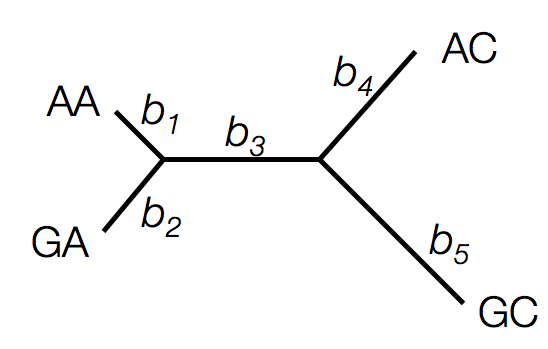
\includegraphics[width=\textwidth]{unrootedTree}
%
%\begin{centering}
%
%
%% Auto-generated from TikzTree.java
%% xScale=3.0 yScale=-1.2566370614359172 offset=0.2
%% scalebar=scalebar{size= 0.1 visible=true}
%% options=[ultra thick]
%% newick=((((A: 0.1, B: 0.2): 0.12, C: 0.3): 0.123, D: 0.4): 0.1234, E: 0.5);
%\begin{tikzpicture}[ultra thick]
%
%\node at (-0.27757, 0.97448) {A};
%\node at (-1.19681, 1.18661) {B};
%\draw (-0.63112, 0.62092) -- (-0.41899, 0.83305);
%\draw (-0.63112, 0.62092) -- (-1.05539, 1.04519);
%\node at (-1.73112, 0.26092) {C};
%\draw (-0.63112, 0.26092) -- (-0.63112, 0.62092);
%\draw (-0.63112, 0.26092) -- (-1.53112, 0.26092);
%\node at (-1.36015, -0.98995) {D};
%\draw (-0.3702, 0) -- (-0.63112, 0.26092);
%\draw (-0.3702, 0) -- (-1.21873, -0.84853);
%\node at (1.7, -0) {E};
%\draw (0, 0) -- (-0.3702, 0);
%\draw (0, 0) -- (1.5, -0);
%
%\draw (0.6996, -0.8485281374238571) -- (0.9996, -0.8485281374238571);
%\node at (0.8496, -0.6485281374238572) {0.1};
%
%\end{tikzpicture}
%
%(c) unrooted tree
%
%\end{centering}
%
%\end{columns}
%
%\medskip{}
%
%\begin{columns}
%
%\column{0.3\textwidth}
%
%\begin{centering}
%
%\scriptsize{((((A, B), C), D), E);}
%
%\end{centering}
%
%\column{0.7\textwidth}
%
%\begin{centering}
%
%\scriptsize{((((A:0.1, B:0.2):0.12, C:0.3):0.123, D:0.4):0.1234, E:0.5);}
%
%\end{centering}
%
%\end{columns}
%
%\bigskip{}
%
%\begin{centering}
%
%branches (edges) and their lengths, nodes, tips (leaves)
%
%\end{centering}
%
%\end{frame}
%
%
%% TIP-LABELED, BIFURCATING ROOTED TREE
%\begin{frame}
%\frametitle{Rooted trees of size 4}
%
%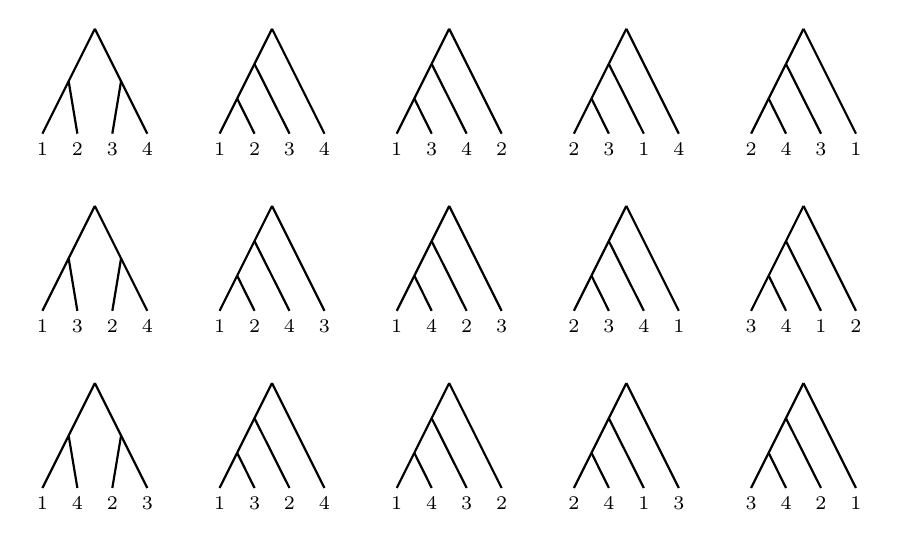
\begin{tikzpicture}[thick,font=\scriptsize]

\node at (0.0, -0.2) {1};
\node at (0.444, -0.2) {2};
\draw (0.0, 0.0) -- (0.333, 0.666);
\draw (0.444, 0.0) -- (0.333, 0.666);
\node at (0.888, -0.2) {3};
\node at (1.332, -0.2) {4};
\draw (0.888, 0.0) -- (0.9990000000000001, 0.666);
\draw (1.332, 0.0) -- (0.9990000000000001, 0.666);
\draw (0.333, 0.666) -- (0.666, 1.332);
\draw (0.9990000000000001, 0.666) -- (0.666, 1.332);
\node at (0.0, -2.45) {1};
\node at (0.444, -2.45) {3};
\draw (0.0, -2.25) -- (0.333, -1.584);
\draw (0.444, -2.25) -- (0.333, -1.584);
\node at (0.888, -2.45) {2};
\node at (1.332, -2.45) {4};
\draw (0.888, -2.25) -- (0.9990000000000001, -1.584);
\draw (1.332, -2.25) -- (0.9990000000000001, -1.584);
\draw (0.333, -1.584) -- (0.666, -0.9179999999999999);
\draw (0.9990000000000001, -1.584) -- (0.666, -0.9179999999999999);
\node at (0.0, -4.7) {1};
\node at (0.444, -4.7) {4};
\draw (0.0, -4.5) -- (0.333, -3.834);
\draw (0.444, -4.5) -- (0.333, -3.834);
\node at (0.888, -4.7) {2};
\node at (1.332, -4.7) {3};
\draw (0.888, -4.5) -- (0.9990000000000001, -3.834);
\draw (1.332, -4.5) -- (0.9990000000000001, -3.834);
\draw (0.333, -3.834) -- (0.666, -3.168);
\draw (0.9990000000000001, -3.834) -- (0.666, -3.168);
\node at (2.25, -0.2) {1};
\node at (2.694, -0.2) {2};
\draw (2.25, 0.0) -- (2.47311, 0.44622);
\draw (2.694, 0.0) -- (2.47311, 0.44622);
\node at (3.138, -0.2) {3};
\draw (2.47311, 0.44622) -- (2.6928900000000002, 0.88578);
\draw (3.138, 0.0) -- (2.6928900000000002, 0.88578);
\node at (3.582, -0.2) {4};
\draw (2.6928900000000002, 0.88578) -- (2.916, 1.332);
\draw (3.582, 0.0) -- (2.916, 1.332);
\node at (2.25, -2.45) {1};
\node at (2.694, -2.45) {2};
\draw (2.25, -2.25) -- (2.47311, -1.80378);
\draw (2.694, -2.25) -- (2.47311, -1.80378);
\node at (3.138, -2.45) {4};
\draw (2.47311, -1.80378) -- (2.6928900000000002, -1.36422);
\draw (3.138, -2.25) -- (2.6928900000000002, -1.36422);
\node at (3.582, -2.45) {3};
\draw (2.6928900000000002, -1.36422) -- (2.916, -0.9179999999999999);
\draw (3.582, -2.25) -- (2.916, -0.9179999999999999);
\node at (2.25, -4.7) {1};
\node at (2.694, -4.7) {3};
\draw (2.25, -4.5) -- (2.47311, -4.05378);
\draw (2.694, -4.5) -- (2.47311, -4.05378);
\node at (3.138, -4.7) {2};
\draw (2.47311, -4.05378) -- (2.6928900000000002, -3.61422);
\draw (3.138, -4.5) -- (2.6928900000000002, -3.61422);
\node at (3.582, -4.7) {4};
\draw (2.6928900000000002, -3.61422) -- (2.916, -3.168);
\draw (3.582, -4.5) -- (2.916, -3.168);
\node at (4.5, -0.2) {1};
\node at (4.944, -0.2) {3};
\draw (4.5, 0.0) -- (4.72311, 0.44622);
\draw (4.944, 0.0) -- (4.72311, 0.44622);
\node at (5.388, -0.2) {4};
\draw (4.72311, 0.44622) -- (4.94289, 0.88578);
\draw (5.388, 0.0) -- (4.94289, 0.88578);
\node at (5.832, -0.2) {2};
\draw (4.94289, 0.88578) -- (5.166, 1.332);
\draw (5.832, 0.0) -- (5.166, 1.332);
\node at (4.5, -2.45) {1};
\node at (4.944, -2.45) {4};
\draw (4.5, -2.25) -- (4.72311, -1.80378);
\draw (4.944, -2.25) -- (4.72311, -1.80378);
\node at (5.388, -2.45) {2};
\draw (4.72311, -1.80378) -- (4.94289, -1.36422);
\draw (5.388, -2.25) -- (4.94289, -1.36422);
\node at (5.832, -2.45) {3};
\draw (4.94289, -1.36422) -- (5.166, -0.9179999999999999);
\draw (5.832, -2.25) -- (5.166, -0.9179999999999999);
\node at (4.5, -4.7) {1};
\node at (4.944, -4.7) {4};
\draw (4.5, -4.5) -- (4.72311, -4.05378);
\draw (4.944, -4.5) -- (4.72311, -4.05378);
\node at (5.388, -4.7) {3};
\draw (4.72311, -4.05378) -- (4.94289, -3.61422);
\draw (5.388, -4.5) -- (4.94289, -3.61422);
\node at (5.832, -4.7) {2};
\draw (4.94289, -3.61422) -- (5.166, -3.168);
\draw (5.832, -4.5) -- (5.166, -3.168);
\node at (6.75, -0.2) {2};
\node at (7.194, -0.2) {3};
\draw (6.75, 0.0) -- (6.97311, 0.44622);
\draw (7.194, 0.0) -- (6.97311, 0.44622);
\node at (7.638, -0.2) {1};
\draw (6.97311, 0.44622) -- (7.19289, 0.88578);
\draw (7.638, 0.0) -- (7.19289, 0.88578);
\node at (8.082, -0.2) {4};
\draw (7.19289, 0.88578) -- (7.416, 1.332);
\draw (8.082, 0.0) -- (7.416, 1.332);
\node at (6.75, -2.45) {2};
\node at (7.194, -2.45) {3};
\draw (6.75, -2.25) -- (6.97311, -1.80378);
\draw (7.194, -2.25) -- (6.97311, -1.80378);
\node at (7.638, -2.45) {4};
\draw (6.97311, -1.80378) -- (7.19289, -1.36422);
\draw (7.638, -2.25) -- (7.19289, -1.36422);
\node at (8.082, -2.45) {1};
\draw (7.19289, -1.36422) -- (7.416, -0.9179999999999999);
\draw (8.082, -2.25) -- (7.416, -0.9179999999999999);
\node at (6.75, -4.7) {2};
\node at (7.194, -4.7) {4};
\draw (6.75, -4.5) -- (6.97311, -4.05378);
\draw (7.194, -4.5) -- (6.97311, -4.05378);
\node at (7.638, -4.7) {1};
\draw (6.97311, -4.05378) -- (7.19289, -3.61422);
\draw (7.638, -4.5) -- (7.19289, -3.61422);
\node at (8.082, -4.7) {3};
\draw (7.19289, -3.61422) -- (7.416, -3.168);
\draw (8.082, -4.5) -- (7.416, -3.168);
\node at (9.0, -0.2) {2};
\node at (9.444, -0.2) {4};
\draw (9.0, 0.0) -- (9.22311, 0.44622);
\draw (9.444, 0.0) -- (9.22311, 0.44622);
\node at (9.888, -0.2) {3};
\draw (9.22311, 0.44622) -- (9.44289, 0.88578);
\draw (9.888, 0.0) -- (9.44289, 0.88578);
\node at (10.332, -0.2) {1};
\draw (9.44289, 0.88578) -- (9.666, 1.332);
\draw (10.332, 0.0) -- (9.666, 1.332);
\node at (9.0, -2.45) {3};
\node at (9.444, -2.45) {4};
\draw (9.0, -2.25) -- (9.22311, -1.80378);
\draw (9.444, -2.25) -- (9.22311, -1.80378);
\node at (9.888, -2.45) {1};
\draw (9.22311, -1.80378) -- (9.44289, -1.36422);
\draw (9.888, -2.25) -- (9.44289, -1.36422);
\node at (10.332, -2.45) {2};
\draw (9.44289, -1.36422) -- (9.666, -0.9179999999999999);
\draw (10.332, -2.25) -- (9.666, -0.9179999999999999);
\node at (9.0, -4.7) {3};
\node at (9.444, -4.7) {4};
\draw (9.0, -4.5) -- (9.22311, -4.05378);
\draw (9.444, -4.5) -- (9.22311, -4.05378);
\node at (9.888, -4.7) {2};
\draw (9.22311, -4.05378) -- (9.44289, -3.61422);
\draw (9.888, -4.5) -- (9.44289, -3.61422);
\node at (10.332, -4.7) {1};
\draw (9.44289, -3.61422) -- (9.666, -3.168);
\draw (10.332, -4.5) -- (9.666, -3.168);

\end{tikzpicture}

%
%\end{frame}
%
%% TIP-LABELED, BIFURCATING LABELLED HISTORIES
%\begin{frame}
%\frametitle{Labeled histories of size 4}
%
%\input{4TaxaHistories.tex}
%
%\end{frame}

\begin{frame}
\frametitle{How many trees are there?}

For $n$ taxa there are

\medskip{}

\begin{centering}

$T^{(R)}_n = (2n - 3)(2n - 5)\dots(3)(1)$ 

\end{centering}

\medskip{}

rooted, binary trees:

\medskip{}

\small{

\begin{tabular}{ccp{0.7\textwidth}} \hline
$n$ & \#trees & \\ \hline
4& 15 &enumerable by hand\\
5& 105 &enumerable by hand on a rainy day\\
6& 945 &enumerable by computer\\
7& 10395 &still searchable very quickly on computer\\
8& 135135 & about the number of hairs on your head\\
9& 2027025 & greater than the population of Auckland\\
10& 34459425 & $\approx$ upper limit for exhaustive search\\
20& $8.20 \times 10^{21}$ & $\approx$ upper limit of branch-and-bound searching\\
48& $3.21 \times 10^{70}$ & $\approx$ the number of particles in the Universe\\
136& $2.11 \times 10^{267}$ & number of trees to choose from in the ``Out of Africa'' data (Vigilante \textit{et al}. 1991)\\
\hline
\end{tabular}

}

\end{frame}

%Section2 The coalescent
\section{The coalescent}

\subimport{../common/slides/}{CoalescentSlides}

%Slide12
\begin{frame}
\frametitle{Constant population size: $N(t)=N_{0}$}

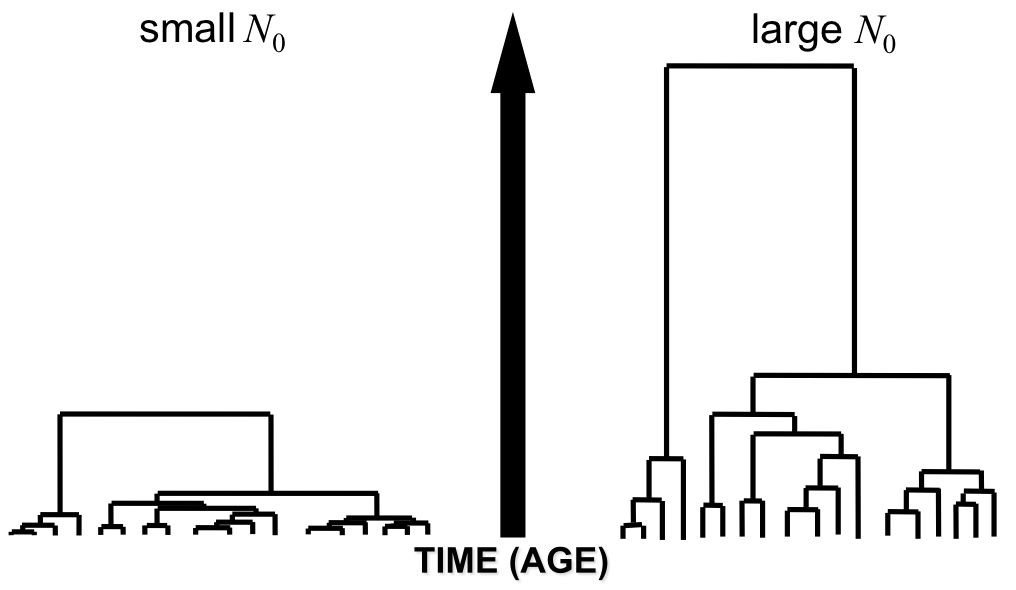
\includegraphics[width=\textwidth]{ConstantPopulationSize}

\end{frame}

%Slide14
\begin{frame}
\frametitle{The coalescent: shapes of genealogies}

\begin{columns}[t]

\column{.5\textwidth}

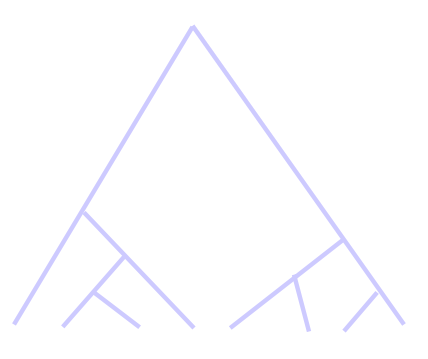
\includegraphics[height=0.45\textheight]{ConstantSize}

\begin{centering}

Constant size

\medskip{}

$N(t) = N_0$

\end{centering}

\column{.5\textwidth}

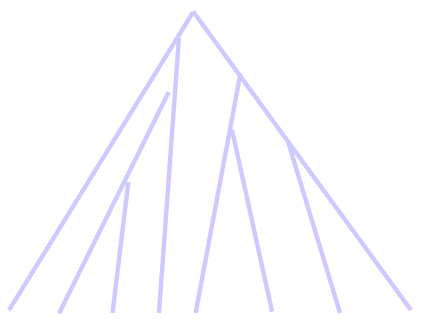
\includegraphics[height=0.45\textheight]{ExponentialGrowth}

\begin{centering}

Exponential growth

\medskip{}

$N(t) = N_{0}exp[-rt]$

\end{centering}

\end{columns}

\medskip{}

\small{The coalescent can be used to convert coalescent times into knowledge about population size and its change though time.}

\end{frame}

%Slide19
\begin{frame}
\frametitle{The coalescent: summary}

\begin{itemize}
	\item The coalescent provides a theory of how population size is related to the distribution of coalescent events in a tree.
	\item Big populations have old trees
	\item Exponentially growing populations have star-like trees
	\item Given a genealogy the most likely population size can be estimated.
	\item Markov chain Monte Carlo (MCMC) can be used to calculate a distribution of trees from the sequence data from which a distribution of population sizes can be estimated.
\end{itemize}

\end{frame}

%\section{Relaxed Phylogenetics}
%
%\subimport{../common/slides/}{Slide_FelLikelihood}
%
%\begin{frame}
%\frametitle{Markov model of nucleotide substitution (Jukes-Cantor)}
%
%\begin{columns}
%
%\column{0.5\textwidth}
%
%\scriptsize{
%\begin{tabular}{|c|cccc|} \hline
%$Q$&To&&& \\ \hline
%From&A&C&G&T \\ \hline
%A&$-3\lambda$&$\lambda$&$\lambda$&$\lambda$\\
%C&$\lambda$&$-3\lambda$&$\lambda$&$\lambda$\\
%G&$\lambda$&$\lambda$&$-3\lambda$&$\lambda$\\
%T&$\lambda$&$\lambda$&$\lambda$&$-3\lambda$\\ \hline
%\end{tabular}
%}
%
%\column{0.5\textwidth}
%
%\begin{centering}
%
%\begin{tikzpicture}[scale=1,every node/.style={fill,orange, circle, text=black},thick] 
%
%\node (A) at (0,0) {A}; 
%\node (C) at (2,2) {C}; 
%\node (G) at (0,2) {G}; 
%\node (T) at (2,0) {T}; 
%
%\draw [<->] (A) to (C);
%\draw [<->] (A) to (G);
%\draw [<->] (A) to (T);
%\draw [<->] (C) to (G);
%\draw [<->] (C) to (T);
%\draw [<->] (G) to (T);
%
%\end{tikzpicture} 
%
%\end{centering}
%
%\end{columns}
%
%\bigskip{}
%
%\begin{columns}
%
%\column{\textwidth}
%
%\small{
%$P(t) = \{p_{ij}(t)\}=e^{Qt}=\begin{bmatrix}
%x_t&y_t&y_t&y_t\\
%y_t&x_t&y_t&y_t\\
%y_t&y_t&x_t&y_t\\
%y_t&y_t&y_t&x_t
% \end{bmatrix},\text{with} 
% \begin{cases} 
%x_t = \frac{1}{4} + \frac{3}{4}e^{-4\lambda t} &  \\
%y_t = \frac{1}{4} - \frac{1}{4}e^{-4\lambda t} & 
%\end{cases}$
%}
%
%\end{columns}
%
%\bigskip{}
%
%$q_{ij}$, $i \neq j$, is the instantaneous rate of change from $i$ to $j$.  The transition probability $p_{ij}(t)$ is the probability that given $i$ now, we observe $j$ time $t$ later.  
%When $t$ is very small, $p_{ij}(t) = \lambda t$, for $i \neq j$.
%
%\end{frame}
%
%
%%\subimport{../common/slides/}{Slide_TreeLandscape}
%
%\subimport{../common/slides/}{Slide_ClockConstraint}
%
%\subimport{../common/slides/}{Slide_ClockModelAssumptions}
%
%\subimport{../common/slides/}{Slide_Calibrations}
%
%%\subimport{../common/slides/}{Slide_FossilAgeGap}
%
%%\subimport{../common/slides/}{Slide_AgeOfPenguins}
%
%\subimport{../common/slides/}{Slide_SampleTimeCalibrations}
%
%\subimport{../common/slides/}{Slide_RelaxedClocks}
%
%\subimport{../common/slides/}{Slide_RelaxedClocksMCMC}
%
%\subimport{../common/slides/}{Slide_RelaxedInfluenza}
%
%\subimport{../common/slides/}{Slide_RelaxedInfluenzaZoom}
%

\subimport{}{SkylineSlides}

\subimport{}{BSPSlides}

%\subimport{}{EBSPSlides}


%SECTION MULTI-SPECIES COALESCENT
\section{Multi-species coalescent}

\begin{frame}[plain]
\frametitle{The murky boundary between population genetics and phylogenetics}

There has been increased interest in analyses of closely related species, where the effect of population genetic processes, such as the coalescent can't be ignored. 

\begin{itemize}
\item Different gene trees can have different topologies due to incomplete lineage sorting
\item Divergence times of species can be overestimated due to ancestral polymorphism
\item Sometimes the exact species identities of individuals are not known
\item Sometimes researchers identify species based on a split in a single gene tree.
\end{itemize}

Enter the multi-species coalescent.

\end{frame}

%Slide26
\begin{frame}[plain]

\begin{columns}[t]

\column{.3\textwidth}

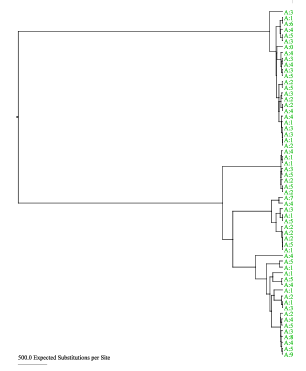
\includegraphics[width=\textwidth]{LineageDrift1}

\bigskip{}

All these patterns are the consequence of ``lineage drift'' within a single population

\column{.3\textwidth}

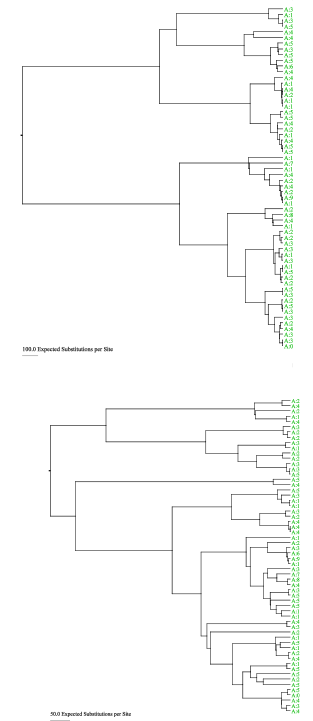
\includegraphics[width=\textwidth]{LineageDrift2}

\column{.3\textwidth}

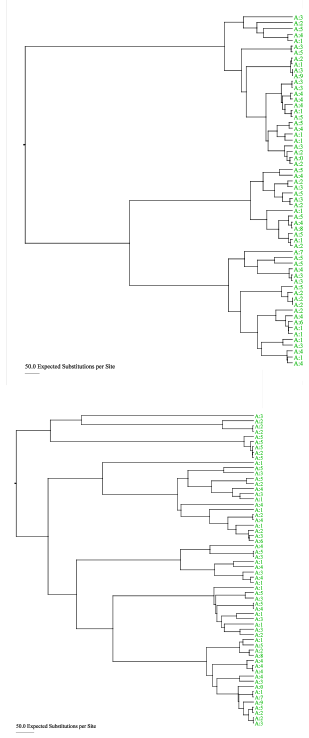
\includegraphics[width=\textwidth]{LineageDrift3}

\end{columns}

\end{frame}

%Slide30
\begin{frame}
\frametitle{Gene trees and species trees}

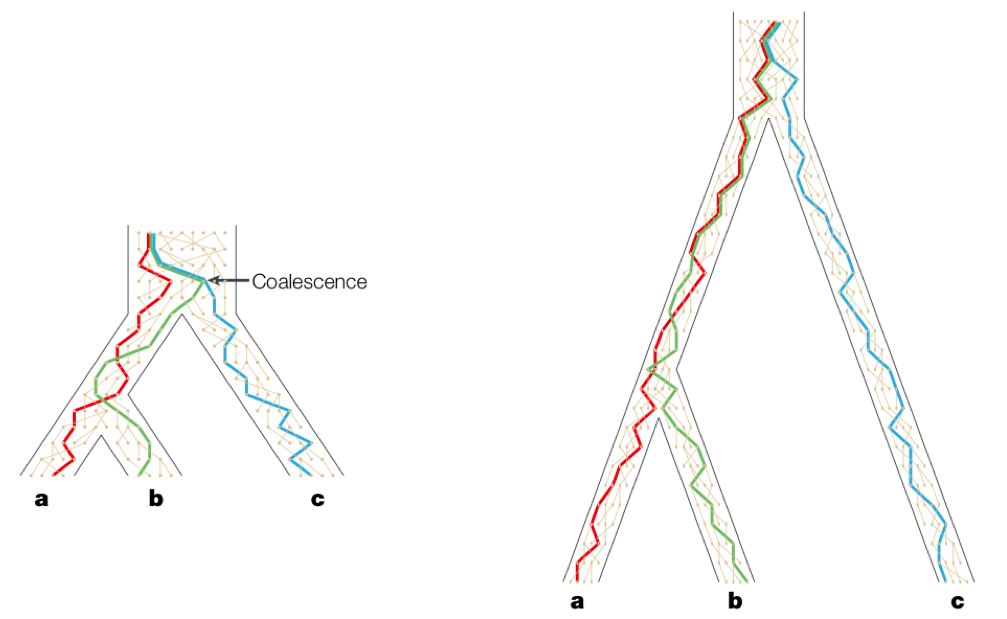
\includegraphics[width=\textwidth]{GeneAndSpeciesTrees}

\end{frame}

%Slide32
\begin{frame}
\frametitle{Why Ancestral Polymorphisms?}

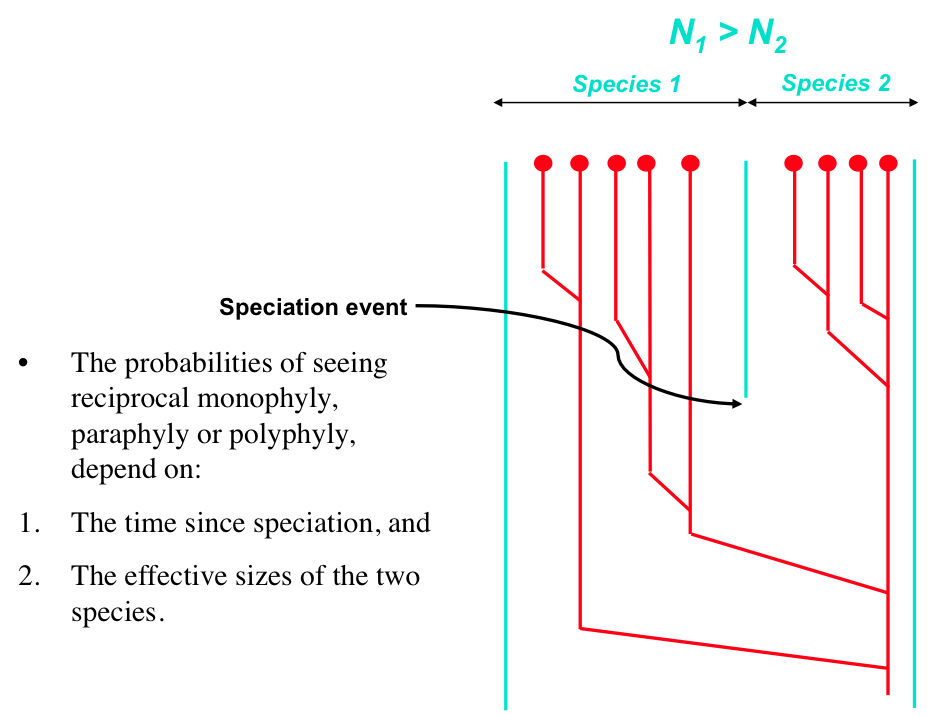
\includegraphics[height=0.8\textheight]{WhyAncestral}

\end{frame}

%Slide33
\begin{frame}
\frametitle{Probabilities of Monophyly, Paraphyly and Polyphyly}

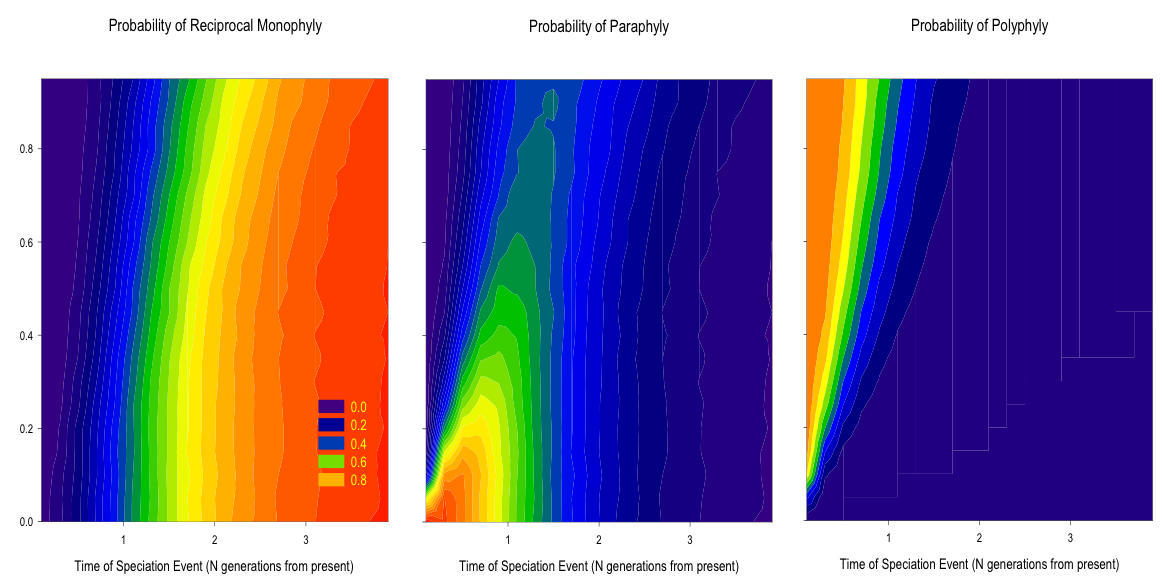
\includegraphics[width=\textwidth]{Phyly}

\end{frame}

%Slide36
\begin{frame}
\frametitle{Problems with estimation of divergence times}

\begin{columns}[t]

\column{.35\textwidth}

\begin{itemize}
	\item Typically we use gene phylogenies to estimate species phylogenies
	\item But divergence time for genes will be longer than that of species.
\end{itemize}

\column{.65\textwidth}

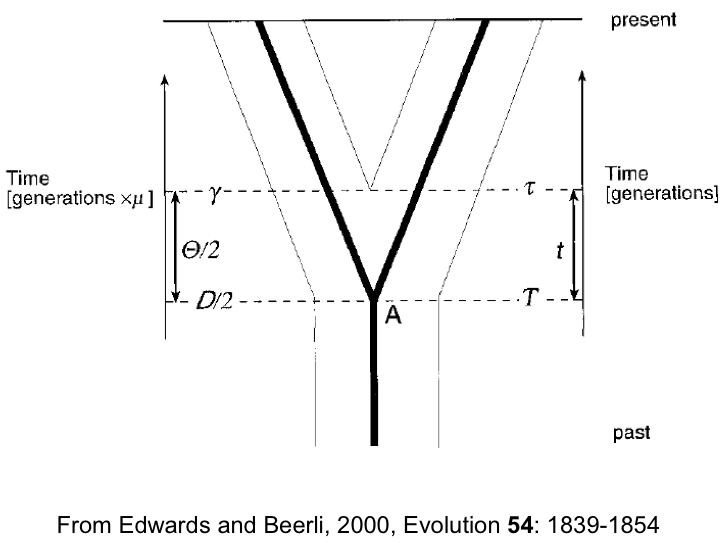
\includegraphics[width=\textwidth]{DivergenceTimes1}

\end{columns}

\end{frame}

%Slide37
\begin{frame}
\frametitle{Problems with estimation of divergence times}

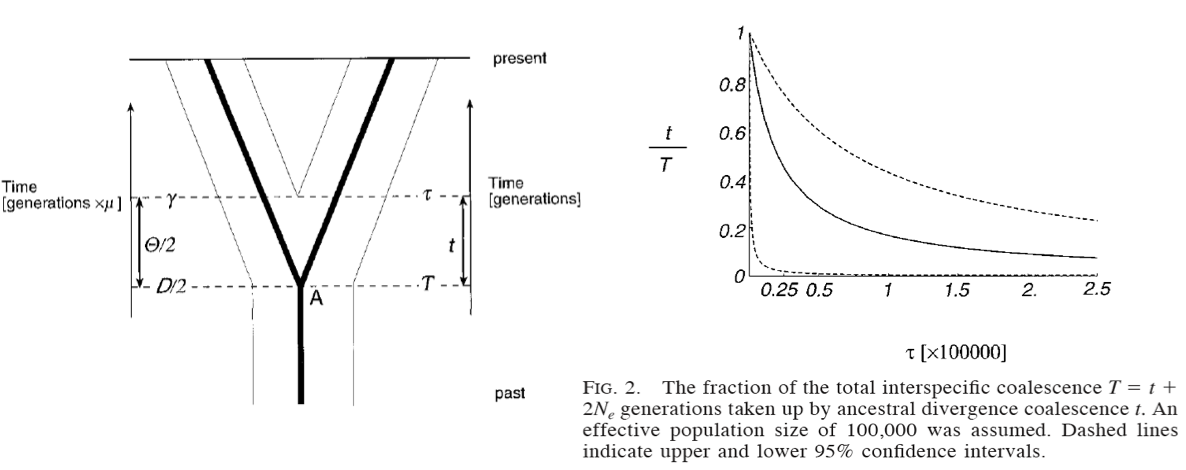
\includegraphics[width=\textwidth]{DivergenceTimes2}

\bigskip{}

\scriptsize{
From Edwards and Beerli, 2000, Evolution \textbf{54}: 1839-1854
}

\end{frame}

% MULTI-SPECIES COALESCENT
\begin{frame}
\frametitle{The multispecies coalescent}

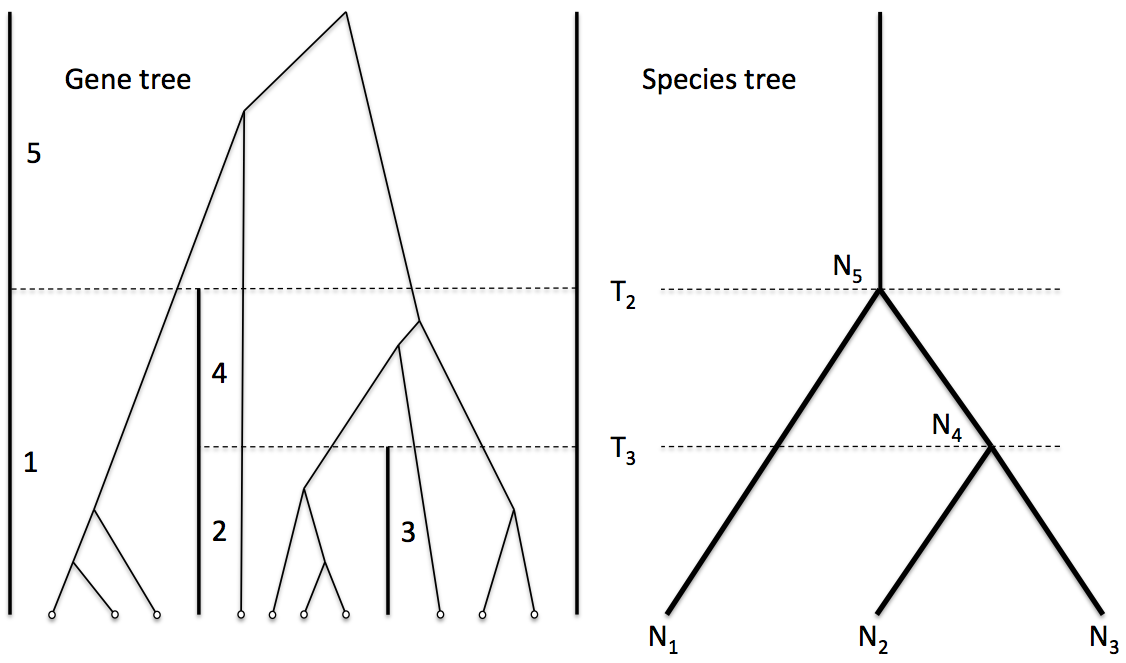
\includegraphics[width=\textwidth]{multispeciesCoalescent/geneTreeSpeciesTree}

\end{frame}

% MULTI-SPECIES COALESCENT
\begin{frame}
\frametitle{Population sizes on a species tree}

Define $N_i$ to be the effective population size at the present for the species $i \in \{1,2,\dots,n\}$, 
and $A_i$ the ancestral effective population of species $i$ at the time of the species origin. 

\bigskip{}

Then for all ancestral species $j \in \{ n+1, n+2, \dots, 2n\}$ (represented by internal branches in the species tree) 
define $N_j = A_{\text{left}(j)} + A_{\text{right}(j)}$, where $\text{left}(i)$ is the left descendent 
of species $i$ and $\text{right}(i)$ is the right descendent species.

\[
A_k \sim \text{Exp}(\Theta), \quad 1 \leq k \leq 2n 
\]

\[
N_i \sim \text{Gamma}(2, \Theta), \quad 1 \leq i \leq n
\]

\[
N_j = A_{\text{left}(j)} + A_{\text{right}(j)}, \quad n < j < 2n 
\]

\end{frame}

% MULTI-SPECIES COALESCENT
\begin{frame}
\frametitle{Population sizes prior}

\begin{centering}

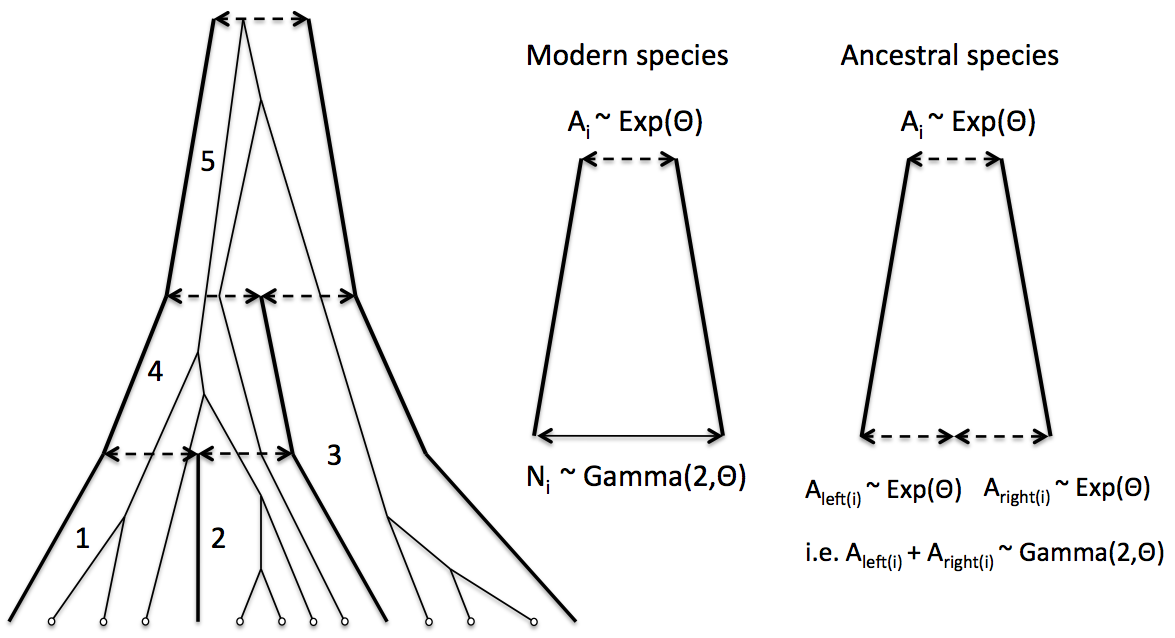
\includegraphics[width=\textwidth]{multispeciesCoalescent/populationPrior}

\end{centering}

\end{frame}

\begin{frame}
\frametitle{Species divergence times prior}

For a species tree of $n$ species, define $T_i$ to be the time at which the species tree goes from having $i$ to $i-1$ species, back in time. Additionally define $\tau_i = T_i - T_{i+1}, i \in \{2,\dots,n-1\}$ and $\tau_n = T_n$.

\medskip{}

The Yule speciation prior supposes a uniform rate species birth ($\lambda$) on all lineages, implying a prior of:

\[
\tau_i \sim \text{Exp}(1/i\lambda)
\]

More complex species tree priors that admit species extinction (Birth-death prior; Gernhard, 2008) and incomplete sampling (Birth-death-sampling; Stadler, 2009) are also possible.

\medskip{}

All of these species tree priors imply a uniform prior on labelled histories.

\end{frame}

% MULTI-SPECIES COALESCENT
\begin{frame}
\frametitle{Coalescent prior for gene trees}

\begin{columns}

\column{0.65\textwidth}

Consider a single species in the species tree, spanned by $k = u-v$ coalescent intervals (and a final interval without a coalescent event). $t_k$ is the time during which there are $k$ lineages. Define $N(s)$ as the population size of this species at time $s$. Define $s_i = \sum_{k=u}^it_k$. The prior density for each interval ending in a coalescent is:

\[
f(t_k) = {\frac{1}{N(s_k)}}  
{\exp\left(-{\int \limits_{s_{k-1}}^{s_k} \frac{\binom{n}{2}}{N(x)} dx }\right)} 
\]

\column{0.35\textwidth}

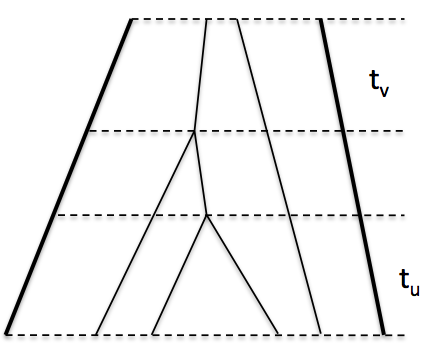
\includegraphics[width=\textwidth]{multispeciesCoalescent/onePopulationCoalescent}

\end{columns}

\end{frame}

% MULTI-SPECIES COALESCENT
\begin{frame}
\frametitle{Coalescent prior for gene trees}

The coalescent prior density for the \textcolor{red}{final interval} that does not end in a coalescent event is:

\[
f(t_v) = {\exp\left(-{\int \limits_{s_{v-1}}^{s_v} \frac{\binom{n}{2}}{N(x)} dx }\right)} 
\]

Define $f_g(g | S)$ to be the total coalescent density for gene tree $g$,  obtained from the product of all the intervals over all species in the species tree (S). 
\end{frame}

% POSTERIOR OF MULTI-SPECIES COALESCENT
\begin{frame}
\frametitle{Posterior probability of multi-species coalescent}

If we additionally define $\color{orange}\Pr(D_g | g)$ as the phylogenetic \textcolor{orange}{likelihood} of the sequence data for gene tree $g$, and $\color{red}P(S | \lambda, \Theta)$ as the \textcolor{red}{prior} on the species tree times and population sizes, then the \textcolor{cyan}{posterior distribution} over gene trees, species tree and other parameters is:

\[
{\color{cyan}P(\mathbf{G},S,\lambda,\Theta | \mathbf{D})} = \frac{1}{\color{green}Z} {\color{orange}\left[\prod_{g\in\mathbf{G}} \Pr(D_g|g)\right]} {\color{red}\left[\prod_{g\in\mathbf{G}} P(g|S)\right]P(S | \lambda, \Theta)P(\lambda)P(\Theta)}
\]

where $\mathbf{G}$ is all the gene trees, $\mathbf{D}$ is all the gene alignments, $\color{red}P(\lambda)$ is the prior for the speciation rate, $\color{red}P(\Theta)$ is the prior on the ancestral population size parameters, and $\color{green}Z = P(\mathbf{D})$ is the unknown normalising constant.

\end{frame}

% MULTI-SPECIES COALESCENT
\begin{frame}
\frametitle{Four gene trees inside a 3-species tree}

\begin{centering}

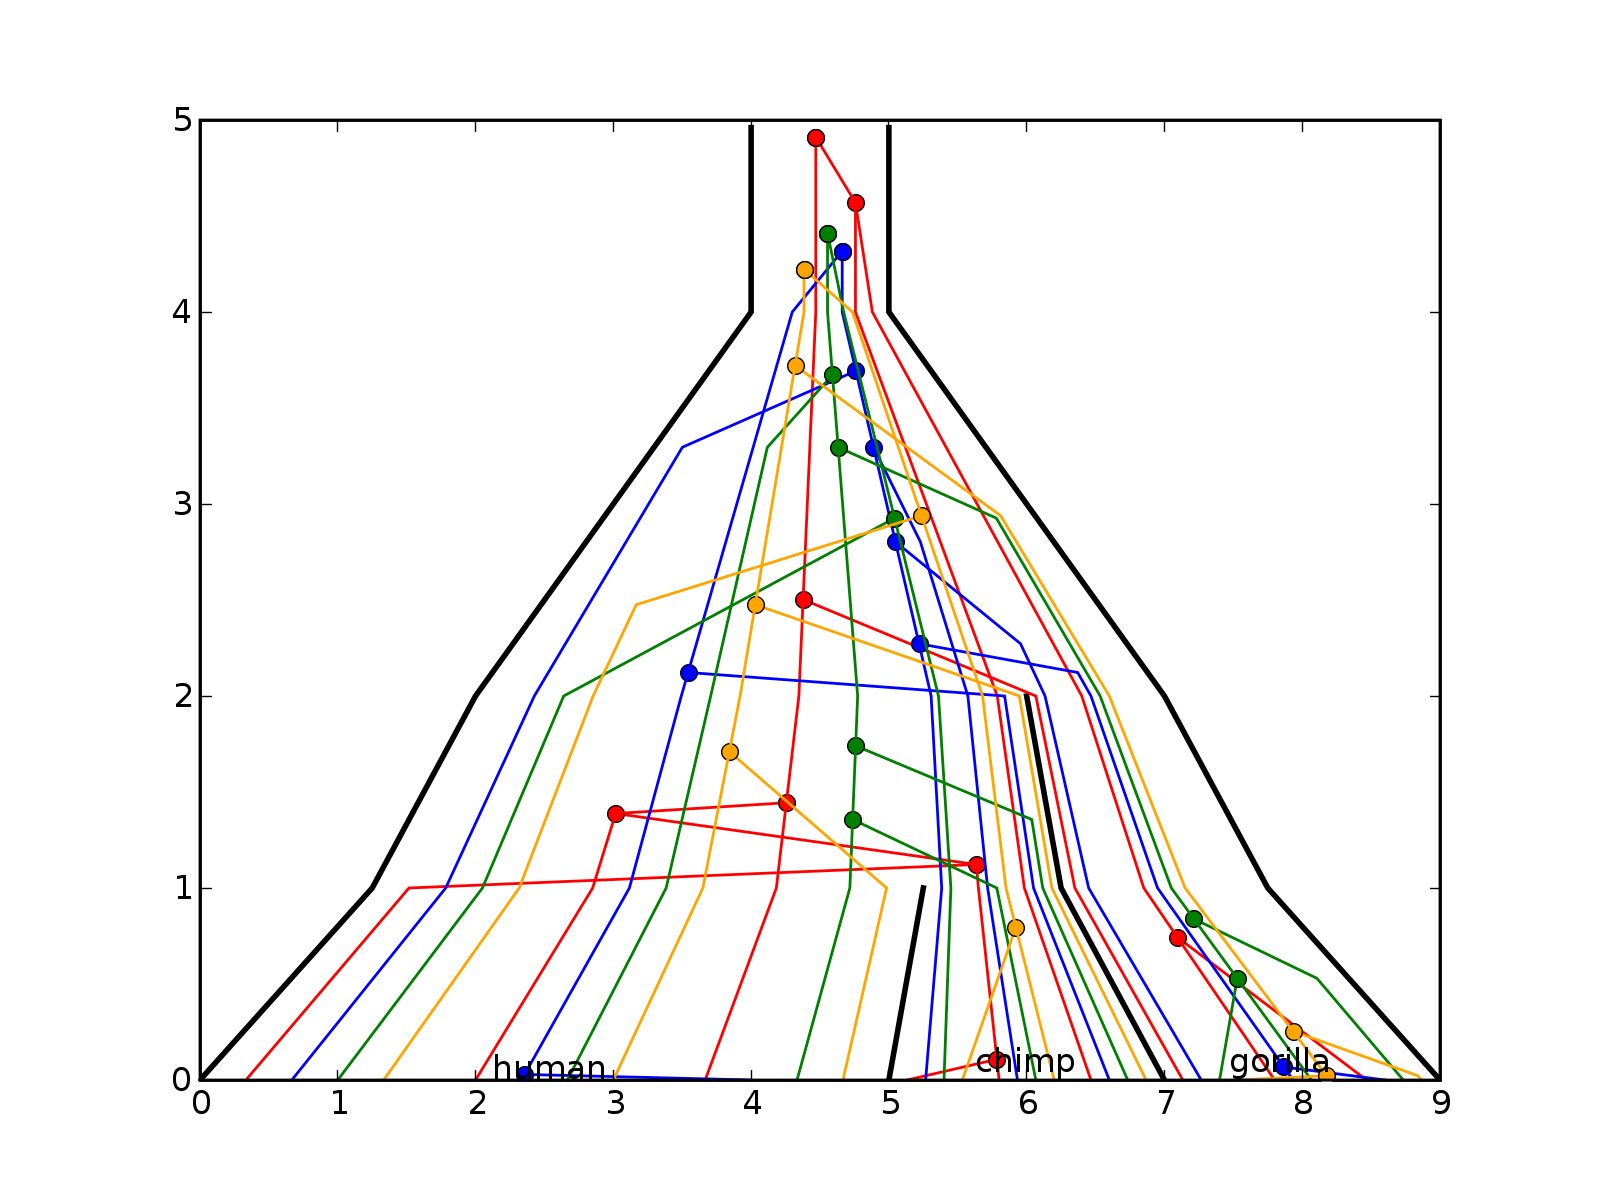
\includegraphics[height=0.9\textheight]{b1_speciesTree}

\end{centering}

\end{frame}

% MULTI-SPECIES COALESCENT
\begin{frame}
\frametitle{A rapid radiation of 7 species}

\begin{centering}

\begin{columns}[t]

\column{0.5\textwidth}

Species tree

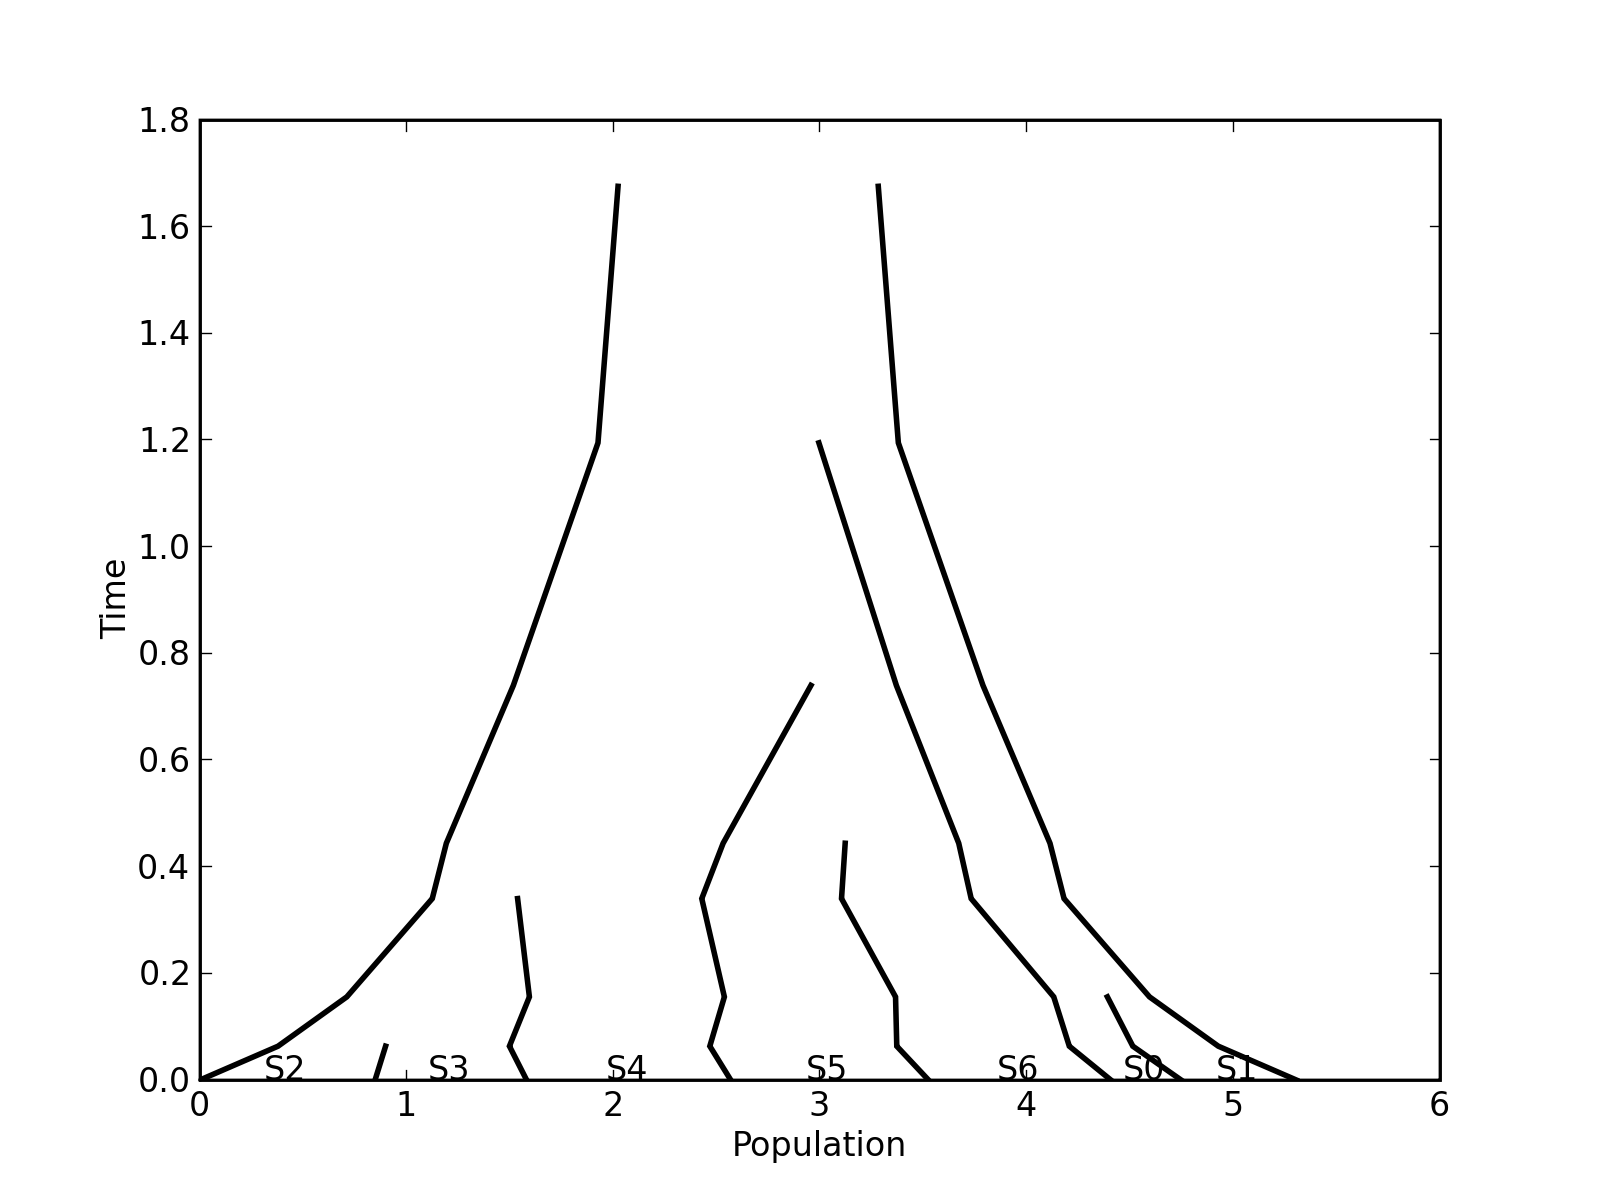
\includegraphics[width=\textwidth]{run1_sptree}

\column{0.5\textwidth}

Species tree and one gene tree

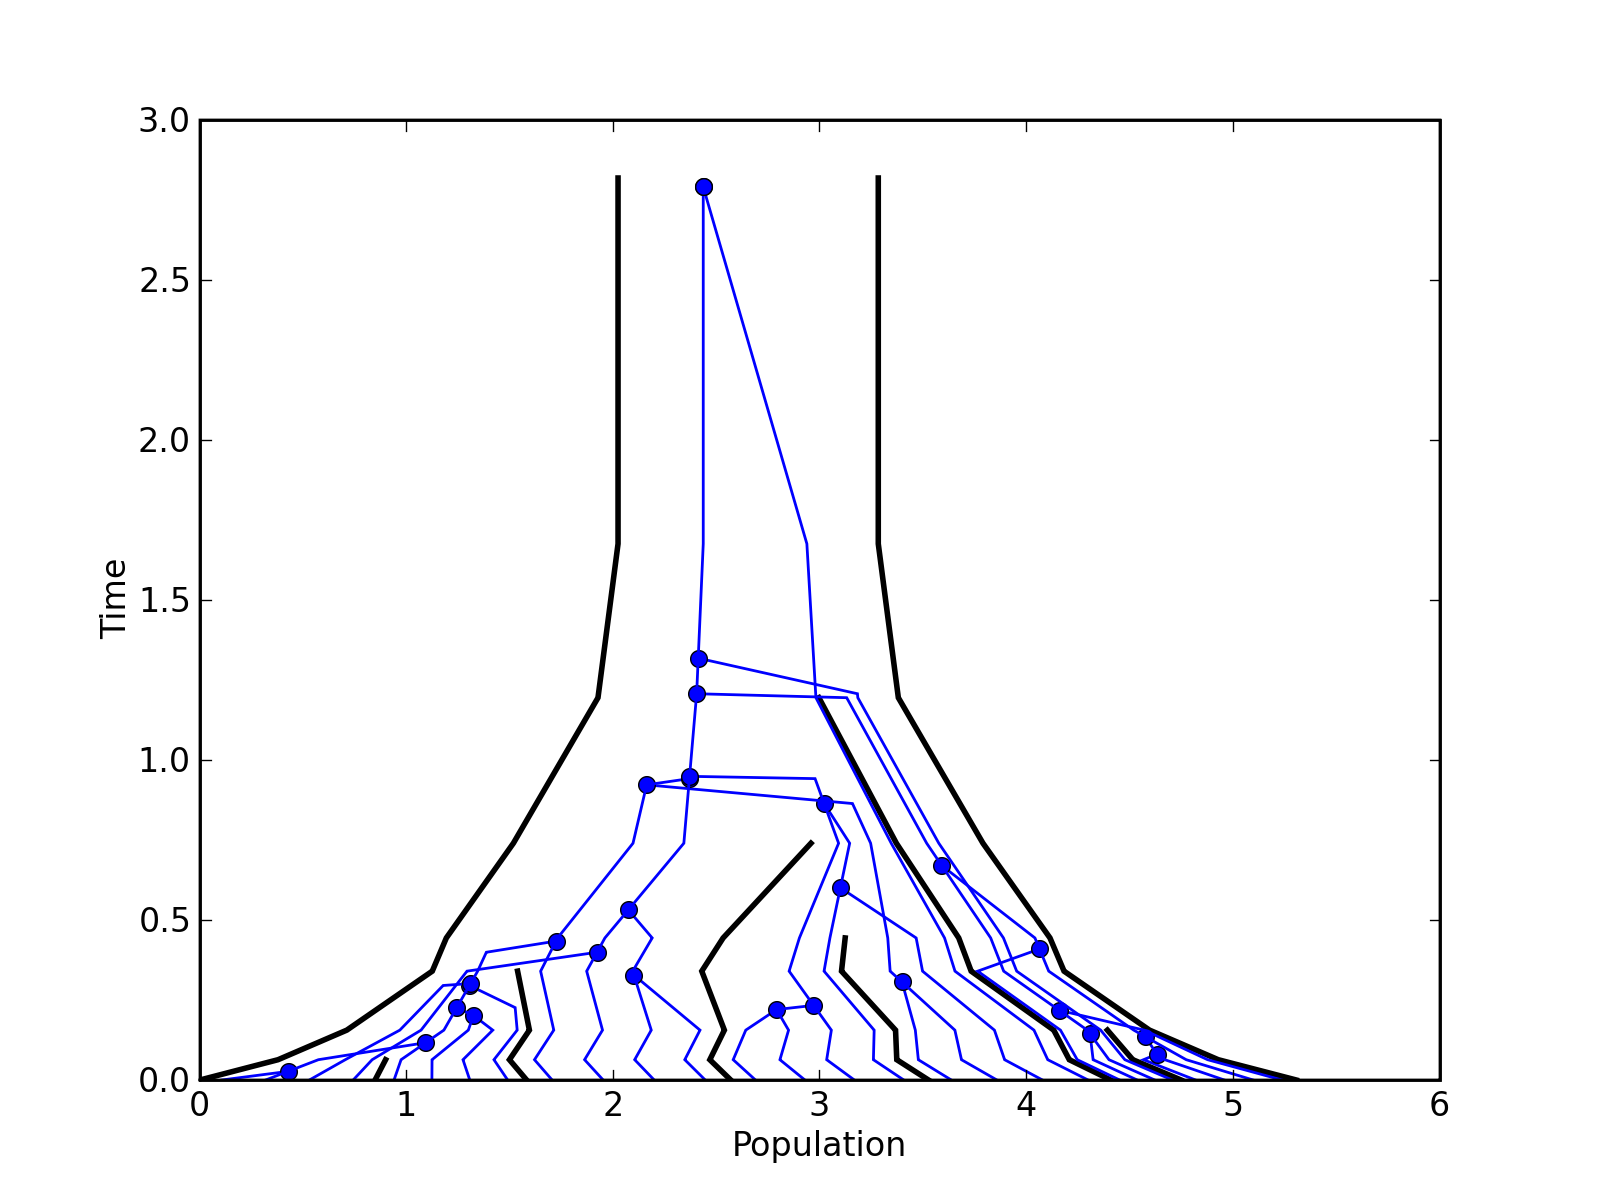
\includegraphics[width=\textwidth]{run1_sptreeand1loci}

\end{columns}

\end{centering}

\end{frame}

% CONCATENATION
\begin{frame}
\frametitle{Gene concatenation - a terrible idea}

\begin{columns}[t]

\column{0.26\textwidth}

\scriptsize{Species tree}

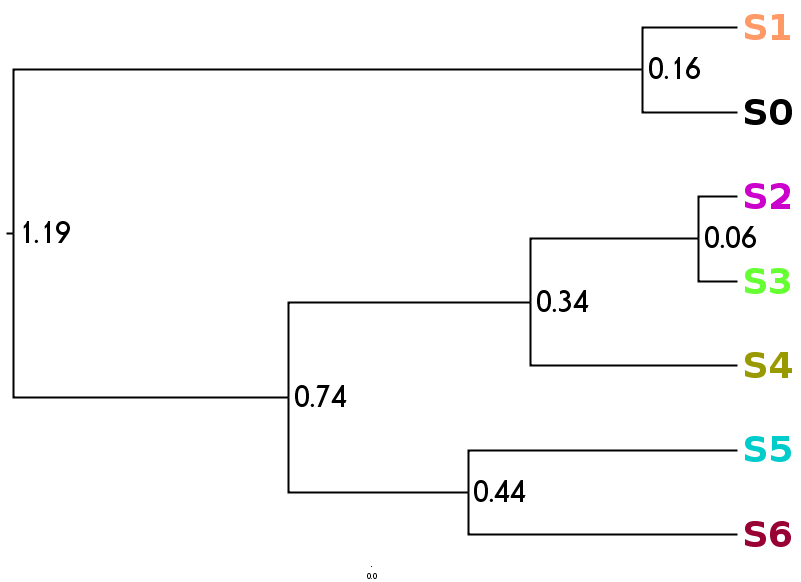
\includegraphics[width=\textwidth]{sp2}

\column{0.74\textwidth}

\scriptsize{``Gene'' tree from concatenated genes}

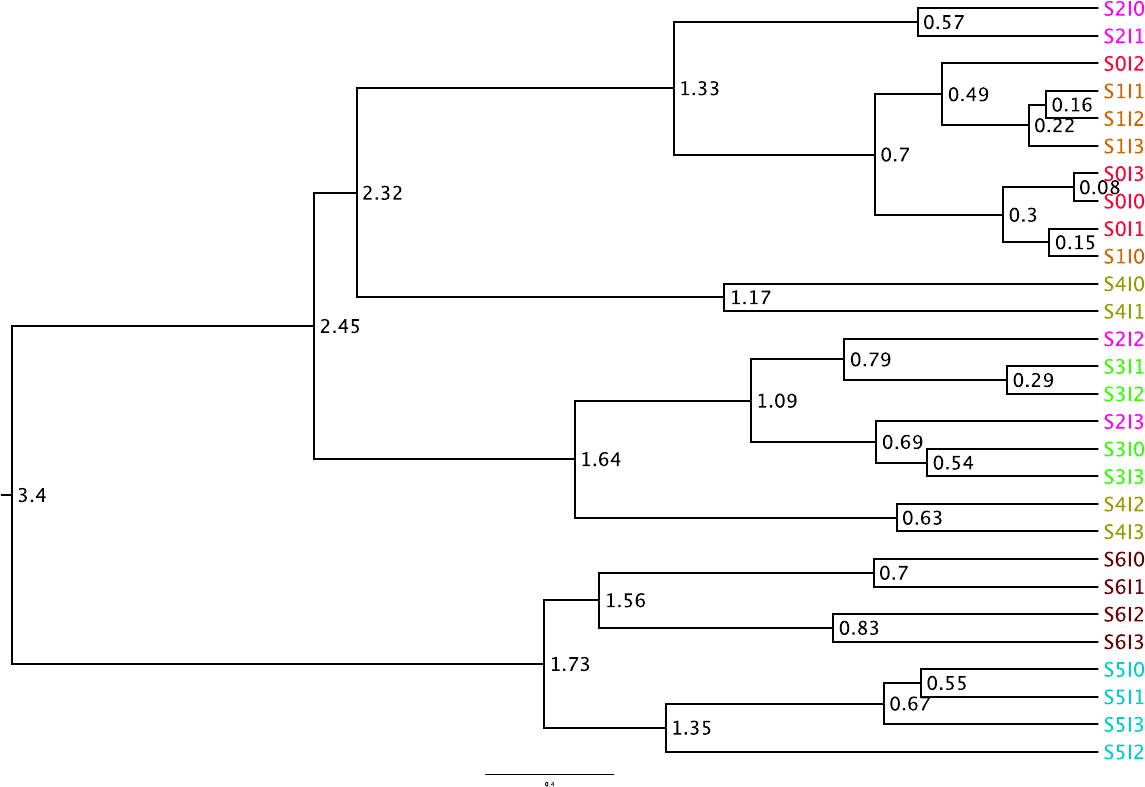
\includegraphics[width=\textwidth]{concatTree}

\end{columns}

\end{frame}

% POCKET GOPHERS 1
\begin{frame}
\frametitle{Pocket Gophers }
\framesubtitle{Data from (Belfiore, 2008)}

\scriptsize{27 individuals, 7 loci (12 from \textit{T. bottae}, 23 from others, 1 from outgroup)}

\bigskip{}

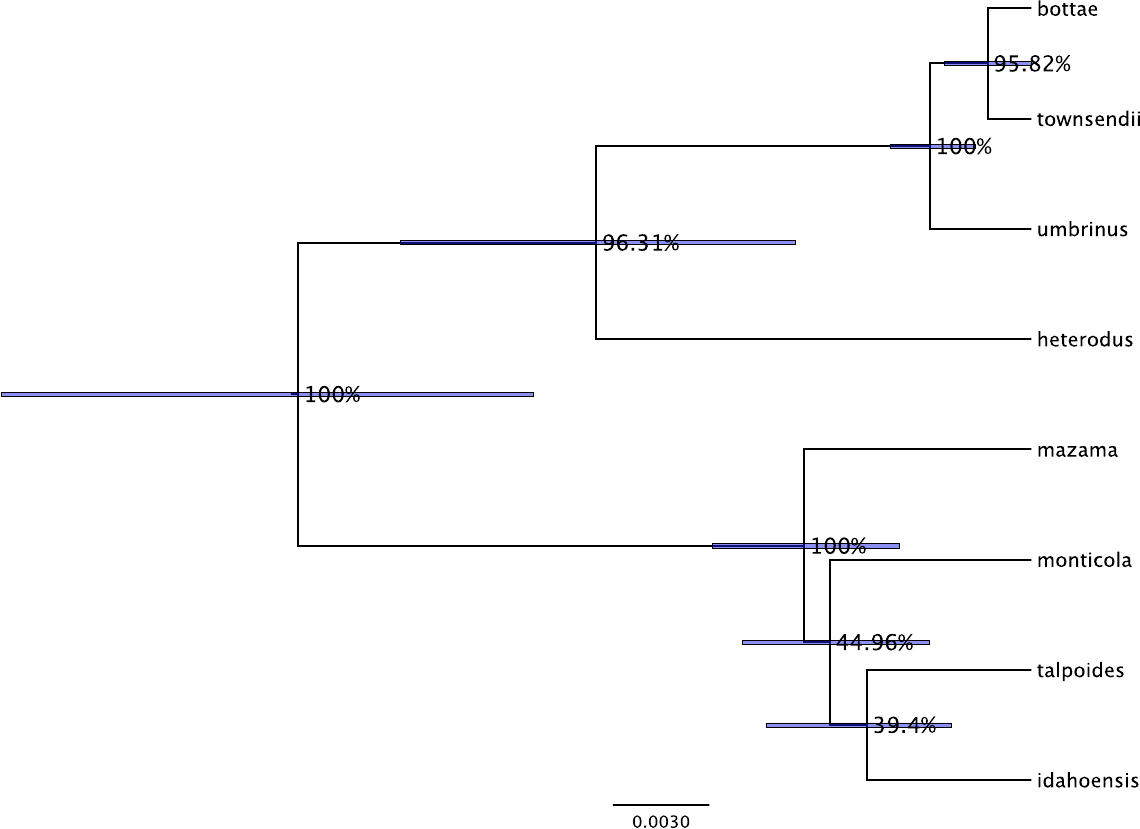
\includegraphics[width=0.8\textwidth]{go3}

\end{frame}

% POCKET GOPHERS 2
\begin{frame}[plain]
\frametitle{Full Bayesian inference under the multi-species coalescent}
\framesubtitle{Data from (Belfiore, 2008), software implemented in BEAST by J. Heled}

\begin{centering}

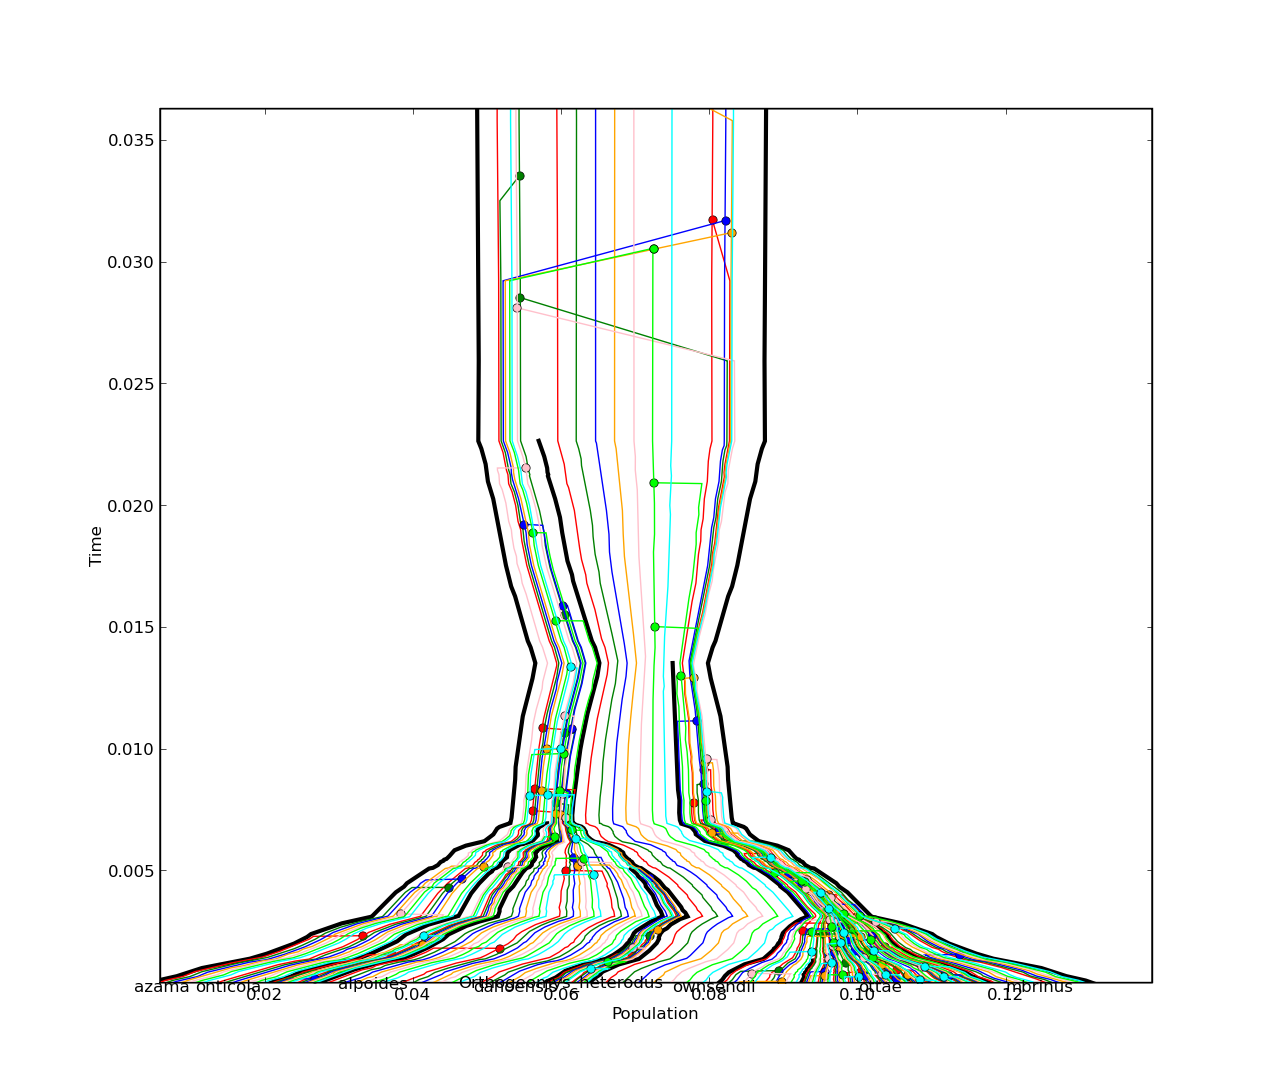
\includegraphics[height=\textheight]{go4}

\end{centering}

\end{frame}

\begin{frame}
\frametitle{Open questions}

\begin{itemize}
\item Are there better priors for the population sizes?
\item What are efficient proposal distributions for MCMC on the multispecies coalescent?
\item What about uncertain species identification?
\begin{itemize}
\item How do we characterize the prior distribution on species associations? (geography, morphology...)
\end{itemize}
\item What about uncertain numbers of species?!
\begin{itemize}
\item How do we characterize the hypothesis space over a species trees with a \textit{random} number of species, and gene tree tips with an uncertain species identity?
\item Reversible-jump, yes, but what proprosal distributions? ;-) What about Bayesian stochastic variable selection?
\end{itemize}
\end{itemize}

\end{frame}

\end{document}
